\documentclass[preprint,12pt,a4paper]{elsarticle}

\usepackage{amssymb}
\usepackage{booktabs}
\usepackage{hyperref}
\usepackage{url}

\setlength{\parindent}{0pt}
\setlength{\emergencystretch}{2em}
\hypersetup{hidelinks}
\graphicspath{{figures/}}
\journal{SoftwareX}

\begin{document}
\renewcommand{\labelenumii}{\arabic{enumi}.\arabic{enumii}}

\begin{frontmatter}

\title{Burrete: Local-first molecular file inspection for macOS, Quick Look, and agent workflows}

\author[ligandpro,innopolis]{Sergei A. Nikolenko\corref{cor1}}
\cortext[cor1]{Corresponding author}
\ead{nikolenko.sergei.chem@gmail.com}
\ead[url]{https://orcid.org/0000-0003-1150-9390}

\address[ligandpro]{Ligand Pro LLC, Bolshoy Boulevard 42, Building 1,
Skolkovo Innovation Center, Moscow 121205, Russia}
\address[innopolis]{Innopolis University, 1 Universitetskaya Street,
Innopolis 420500, Russia}

\begin{abstract}
Burrete is an open-source, local-first workspace for inspecting molecular
artifacts on macOS. It combines Finder Quick Look, a Tauri desktop workspace,
a source-built iPhone preview target, and typed agent interfaces. Rather than
introducing a molecular graphics or modeling algorithm, Burrete routes local
documents to established components: Mol* for interactive structures and
MolViewSpec scenes, RDKit for molecule collections, Ketcher for sketching,
optional \texttt{xyzrender} for SVG output, VESTA handoff, and bounded
text/metadata fallbacks. This integration supports rapid checks of structures,
pose collections, trajectories, quantum-chemistry inputs, and workflow outputs
before heavier analysis. Version 1.0.22 is released under the MIT License with
source, documentation, sample files, and macOS binaries on GitHub.
\end{abstract}

\begin{keyword}
molecular visualization \sep research software \sep computational chemistry
\sep cheminformatics \sep Quick Look \sep agent workflows
\end{keyword}

\end{frontmatter}

\section*{Required Metadata}

\section*{Current code version}

\begin{table}[!ht]
\begin{tabular}{|l|p{5.85cm}|p{5.85cm}|}
\hline
\textbf{Nr.} & \textbf{Code metadata description} &
\textbf{Please fill in this column} \\
\hline
C1 & Current code version & v1.0.22 \\
\hline
C2 & Permanent GitHub link to code/repository used for this code version &
\url{https://github.com/SergeiNikolenko/Burrete/tree/softwarex-v1.0.22} \\
\hline
C3 & Legal Code License & MIT License \\
\hline
C4 & Code versioning system used & Git \\
\hline
C5 & Software code languages, tools, and services used &
TypeScript, JavaScript, Rust, Swift, HTML/CSS, shell; Tauri 2; Mol* 5.7.0;
RDKit 2025.03.4; Ketcher 3.12/3.15 \\
\hline
C6 & Compilation requirements, operating environments \& dependencies &
macOS 12 or later; Bun and Rust/Tauri for the desktop source build; Xcode for
the Quick Look extension and source-built iPhone target. Mol*, RDKit, and
Ketcher assets are bundled. \texttt{xyzrender} and VESTA are optional external
tools. \\
\hline
C7 & If available Link to developer documentation/manual &
\url{https://github.com/SergeiNikolenko/Burrete/blob/softwarex-v1.0.22/README.md} \\
\hline
C8 & Support email for questions & \url{nikolenko.sergei.chem@gmail.com} \\
\hline
\end{tabular}
\caption{Code metadata (mandatory).}
\label{tab:code-metadata}
\end{table}

\textbf{Main text}

\begin{enumerate}

\item \textbf{Motivation and significance}

Computational chemistry, structural biology, docking, and cheminformatics
workflows create heterogeneous local artifacts: coordinate files, ligand
collections, docking poses, trajectories, quantum-chemistry inputs and outputs,
topologies, logs, and generated reports. Before a researcher can interpret a
result, a smaller question often has to be answered: does this file contain the
expected structure, set of molecules, frames, or workflow state? Repeatedly
opening a full modeling application for that check interrupts the file-oriented
workflow, while a generic operating-system preview usually lacks molecular
semantics.

Established applications and libraries already solve the difficult scientific
and graphics problems. ChimeraX and Coot support structural analysis,
model-building, and refinement \cite{chimerax,coot}; VMD and PyMOL are broad
molecular-visualization environments \cite{vmd,pymol}; Avogadro supports
molecular editing and computational-chemistry workflows \cite{avogadro}; and
Open Babel and RDKit provide conversion and cheminformatics capabilities
\cite{openbabel,rdkit}. Web components such as Mol*, NGL, Jmol/JSmol, and
3Dmol.js make molecular visualization embeddable in applications
\cite{molstar,ngl,jmol,threedmol}.

Burrete addresses a narrower integration problem: it gives the same local
artifact an operating-system preview, a persistent desktop workspace, an
explicit renderer route, and---when requested---a typed agent session. A typical
user selects a molecular file in Finder and presses Space for a Quick Look
preview, or opens a project folder in the desktop application to compare files
in tabs and docked panels. The contribution is therefore not a new molecular
graphics, cheminformatics, docking, or simulation algorithm. It is a documented
inspection and handoff layer that reduces friction between file generation and
scientific analysis.

\item \textbf{Software description}

\begin{enumerate}

\item \textit{Software architecture.}

Figure~\ref{fig:architecture} summarizes the architecture. A checked-in format
registry defines document types and routing policy. Three user-facing
applications consume that policy: a Swift Quick Look extension following
Apple's extension model \cite{applequicklook}, a React desktop workspace hosted
by Tauri \cite{tauri}, and an experimental iPhone preview target built from
source. The desktop and Quick Look surfaces package their own runtime artifacts
and caches; they are tested separately because a successful browser preview
does not establish that macOS has registered the native extension.

\begin{figure}[htbp]
  \centering
  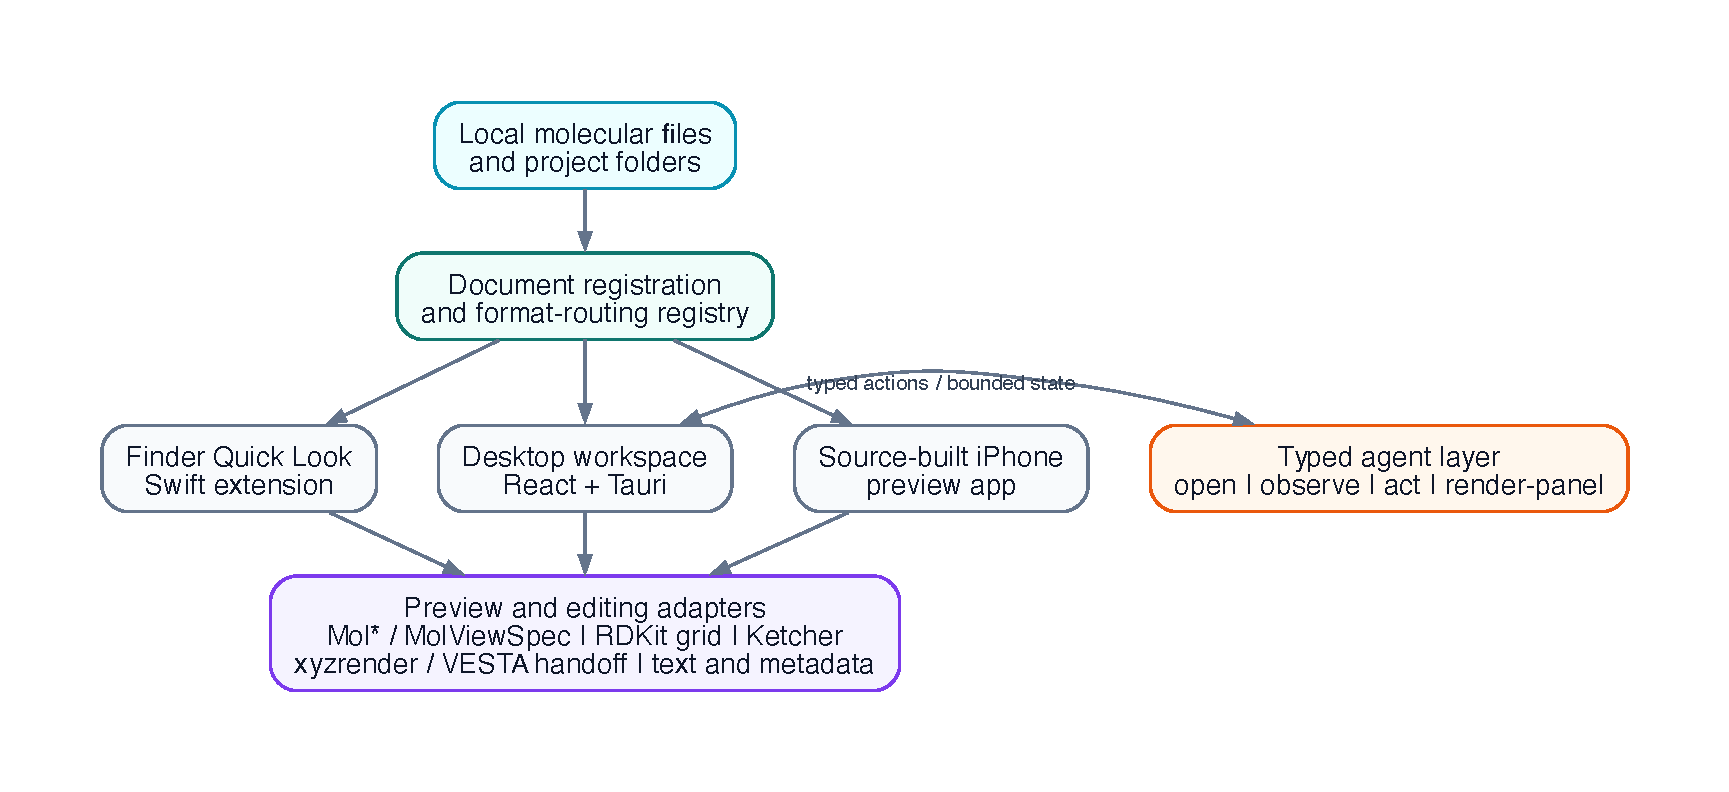
\includegraphics[width=\linewidth]{Figure_1_architecture.pdf}
  \caption{Burrete architecture. A shared document and format registry routes
  local files to native or desktop surfaces and then to explicit preview or
  editing adapters. The agent layer exchanges typed actions and bounded state
  with a workspace session.}
  \label{fig:architecture}
\end{figure}

The preview adapters make component ownership explicit. Mol* 5.7.0 renders
supported coordinate files and MolViewSpec scenes
\cite{molstar,molviewspec}; the packaged RDKit 2025.03.4 WebAssembly runtime
parses and depicts molecule collections \cite{rdkit}; and Ketcher provides
small-molecule and reaction editing \cite{ketcher}. Optional
\texttt{xyzrender} produces SVG-oriented molecular graphics
\cite{xyzrender}, while VESTA can be invoked for compatible crystal,
volumetric, and quantum-chemistry artifacts \cite{vesta}. Files without enough
standalone structural information remain available through text or metadata
views. OpenMM is an example of an upstream simulation ecosystem whose
coordinate and state artifacts can be inspected; Burrete does not execute the
simulation \cite{openmm}.

The agent platform is a separate typed boundary over the workspace. Repository
commands expose \texttt{open}, \texttt{observe}, \texttt{act}, and
\texttt{render-panel}. Observations report bounded state such as active and
open documents, viewer readiness, panels, selection, and the last action
result. Actions are explicit discriminated operations rather than unrestricted
screen control or arbitrary file injection.

\item \textit{Software functionalities.}

The main functions are:

\begin{itemize}
  \item native registration and Finder Quick Look for supported local
  molecular documents;
  \item a tabbed desktop workspace with project folders, recent files, command
  search, renderer switching, and text fallbacks;
  \item Mol* previews for common structure formats and declarative MVSJ/MVSX
  scenes;
  \item RDKit-backed grids for SDF, SD, SMILES, CSV, and TSV collections with
  search, sorting, SMARTS filtering/highlighting, selection, append/merge, and
  export;
  \item Ketcher small-molecule and reaction sketching, with handoff to preview
  and collection workflows;
  \item optional \texttt{xyzrender} and VESTA routing for formats and tasks
  better handled by those external applications;
  \item inspection of trajectory, topology, FEP-network, quantum-chemistry,
  OpenMM, Amber, and CHARMM artifacts when sufficient standalone or paired
  context exists, otherwise a text or metadata view; and
  \item typed browser or desktop sessions for bounded agent-assisted inspection.
\end{itemize}

These functions intentionally preserve boundaries. Burrete does not claim
automatic chemical interpretation, property prediction, scoring, structure
refinement, trajectory analysis, or complete direct rendering of every
registered extension.

\end{enumerate}

\item \textbf{Illustrative examples}

The first example is fast structure triage. Selecting a PDB, mmCIF, SDF, or XYZ
document in Finder invokes the registered Quick Look path. Opening the same
document in the desktop workspace adds persistent tabs, project navigation,
renderer controls, selection, and comparison panels. Figure~\ref{fig:workspace}
shows a PDB structure in the Mol*-based workspace. The user can verify the
macromolecular assembly and ligand context, then keep that view mounted while
inspecting related project files.

\begin{figure}[htbp]
  \centering
  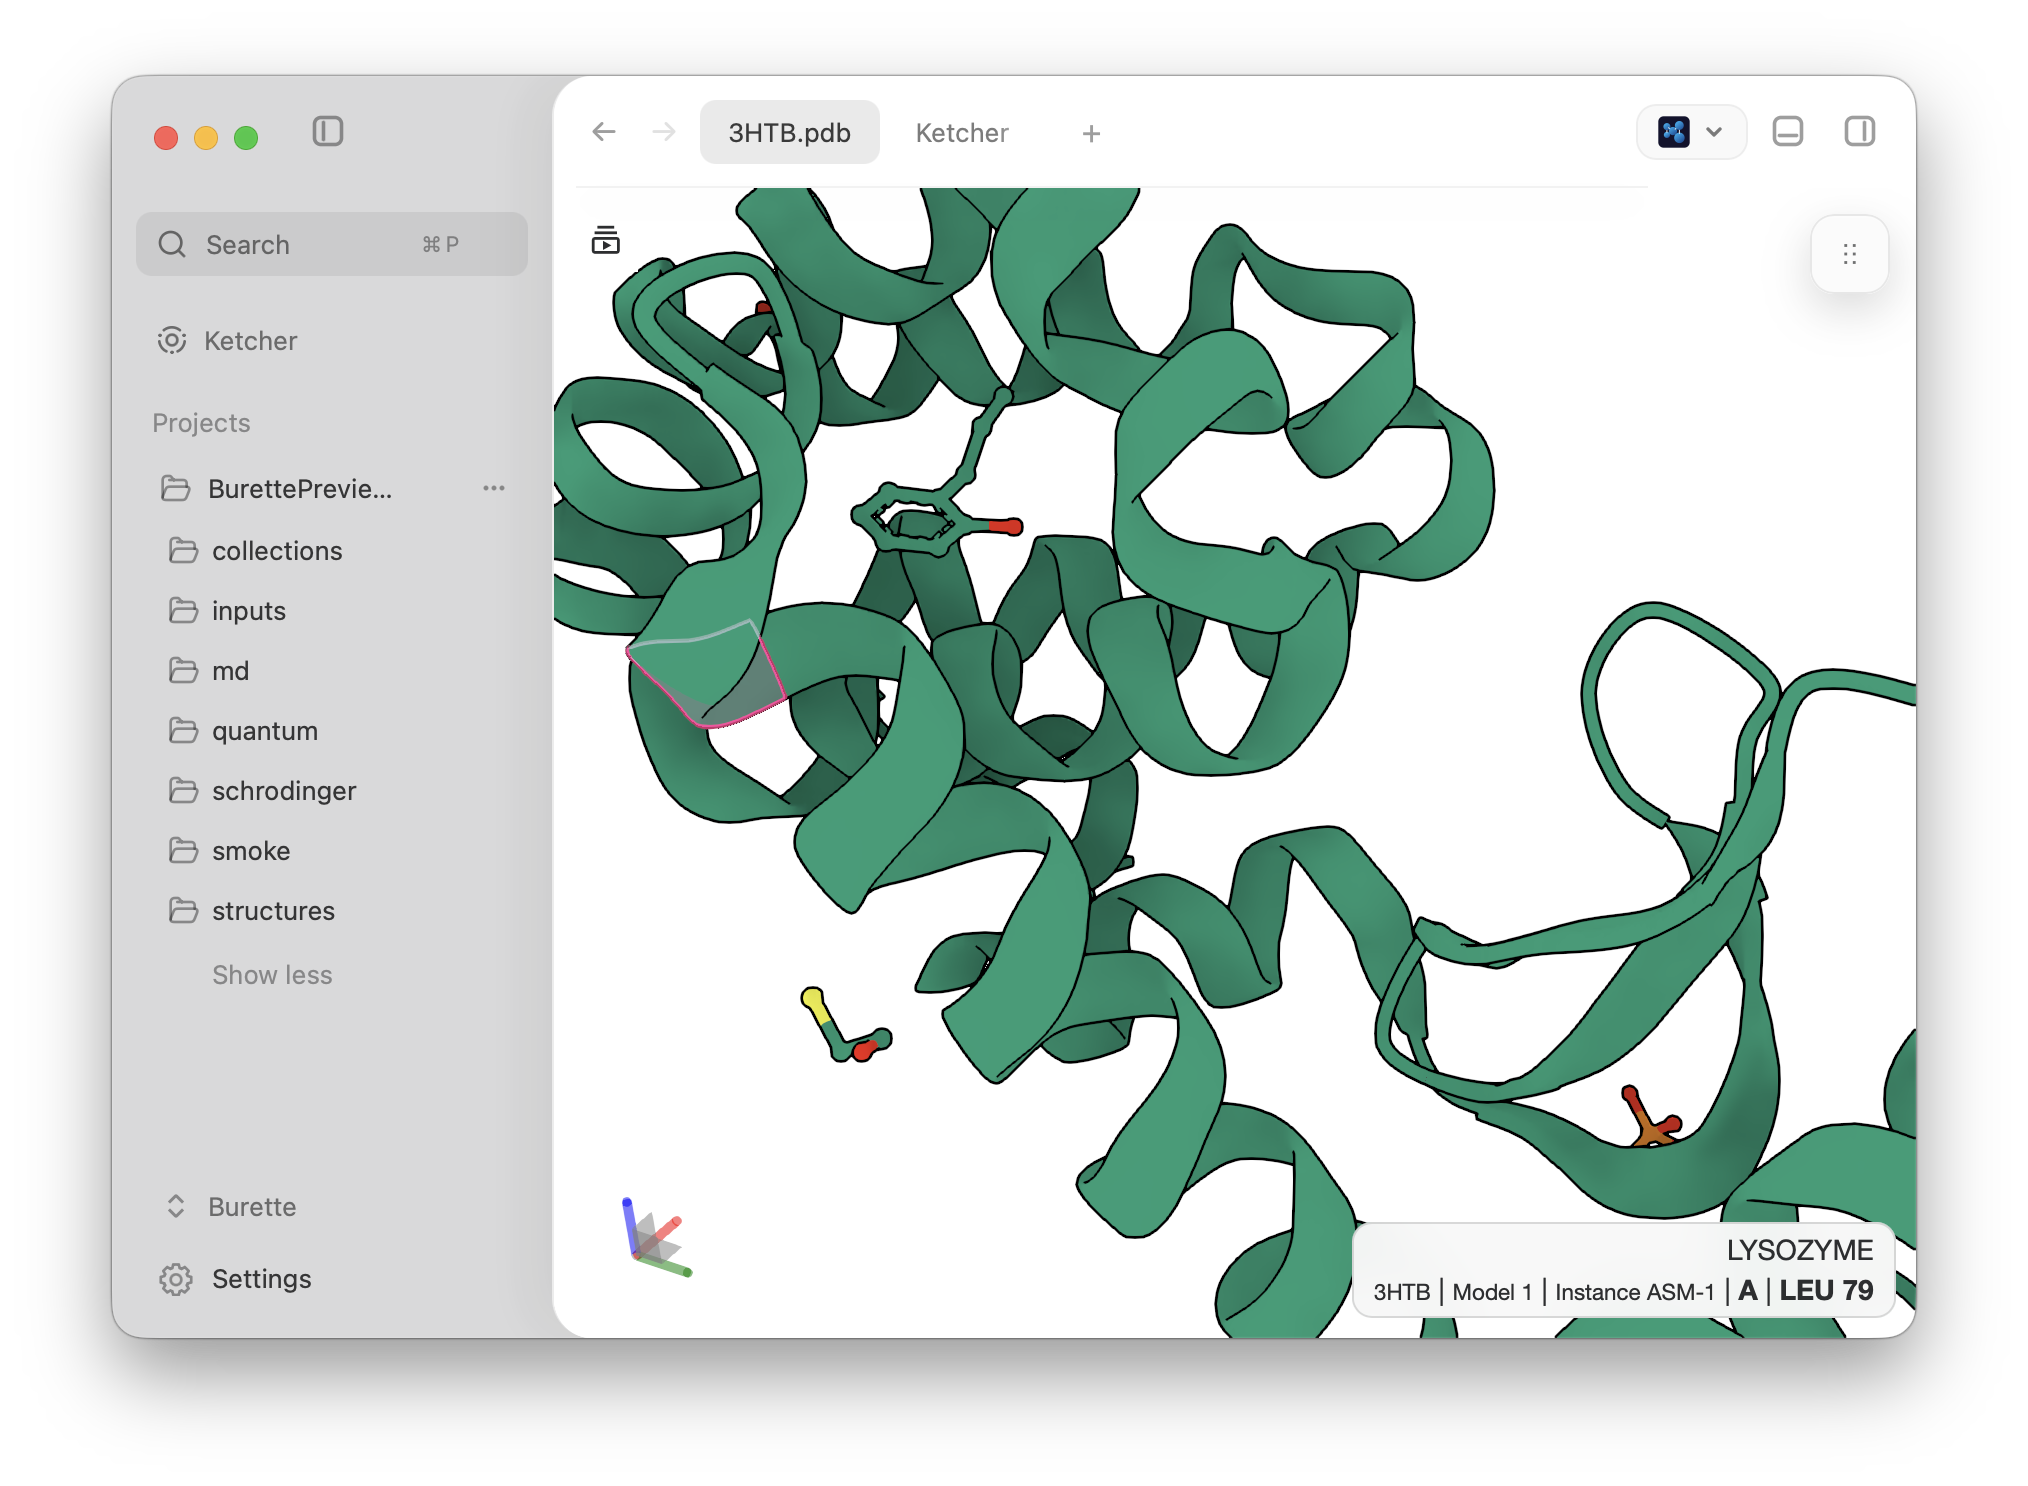
\includegraphics[width=0.92\linewidth]{Figure_2_workspace.png}
  \caption{Desktop workspace displaying PDB entry 3HTB with the Mol*-based
  viewer, project navigation, tabbed documents, and atom-level selection.}
  \label{fig:workspace}
\end{figure}

The second example is collection triage. An SDF, SMILES, CSV, or TSV file opens
as a table of molecule records. Depictions and source fields remain together;
the user can search or sort, apply a SMARTS filter, select records, edit a row
in Ketcher, preview it in Mol*, or export a subset. Figure~\ref{fig:grid} shows
the context actions for a selected SDF record. This path is useful for checking
generated libraries and docking-input collections before launching downstream
computations.

\begin{figure}[htbp]
  \centering
  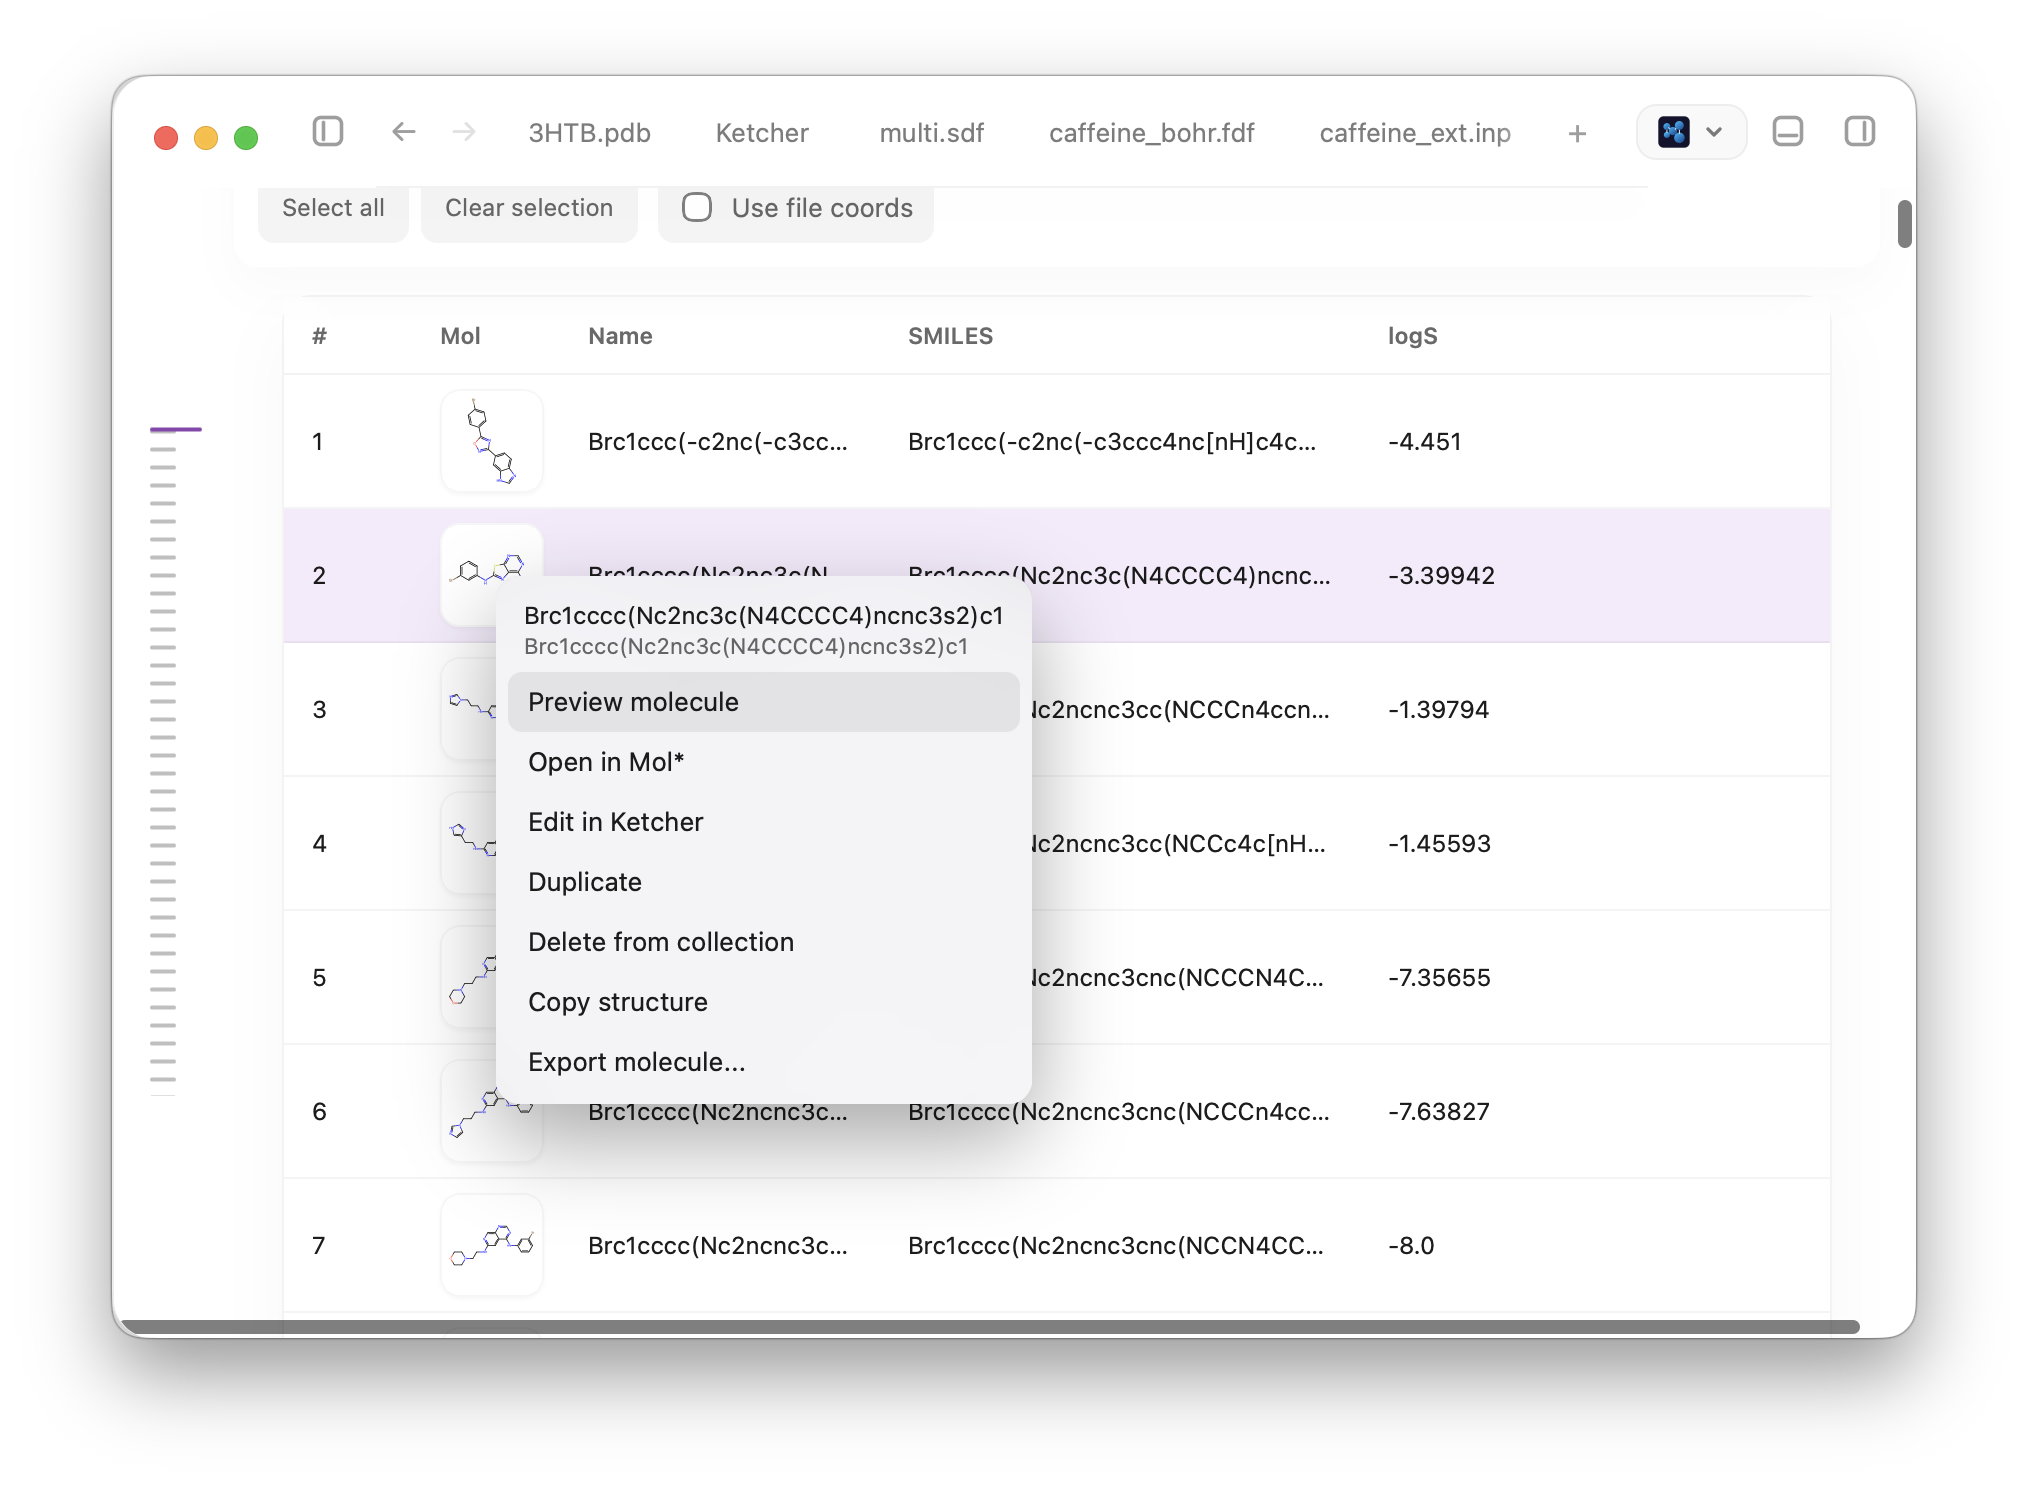
\includegraphics[width=0.88\linewidth]{Figure_3_collection_grid.png}
  \caption{RDKit-backed SDF collection grid. Molecular depictions, source
  properties, selection, preview, editing, and export remain in one local
  workspace.}
  \label{fig:grid}
\end{figure}

The third example is explicit external rendering. When
\texttt{xyzrender} is installed, a compatible XYZ or quantum-chemistry artifact
can be routed to it without losing the surrounding project context.
Figure~\ref{fig:xyzrender} shows the SVG preview and renderer presets in a
docked panel. The same principle applies to VESTA handoff: Burrete owns file
discovery and routing, while the specialized external program owns the
scientific visualization.

\begin{figure}[htbp]
  \centering
  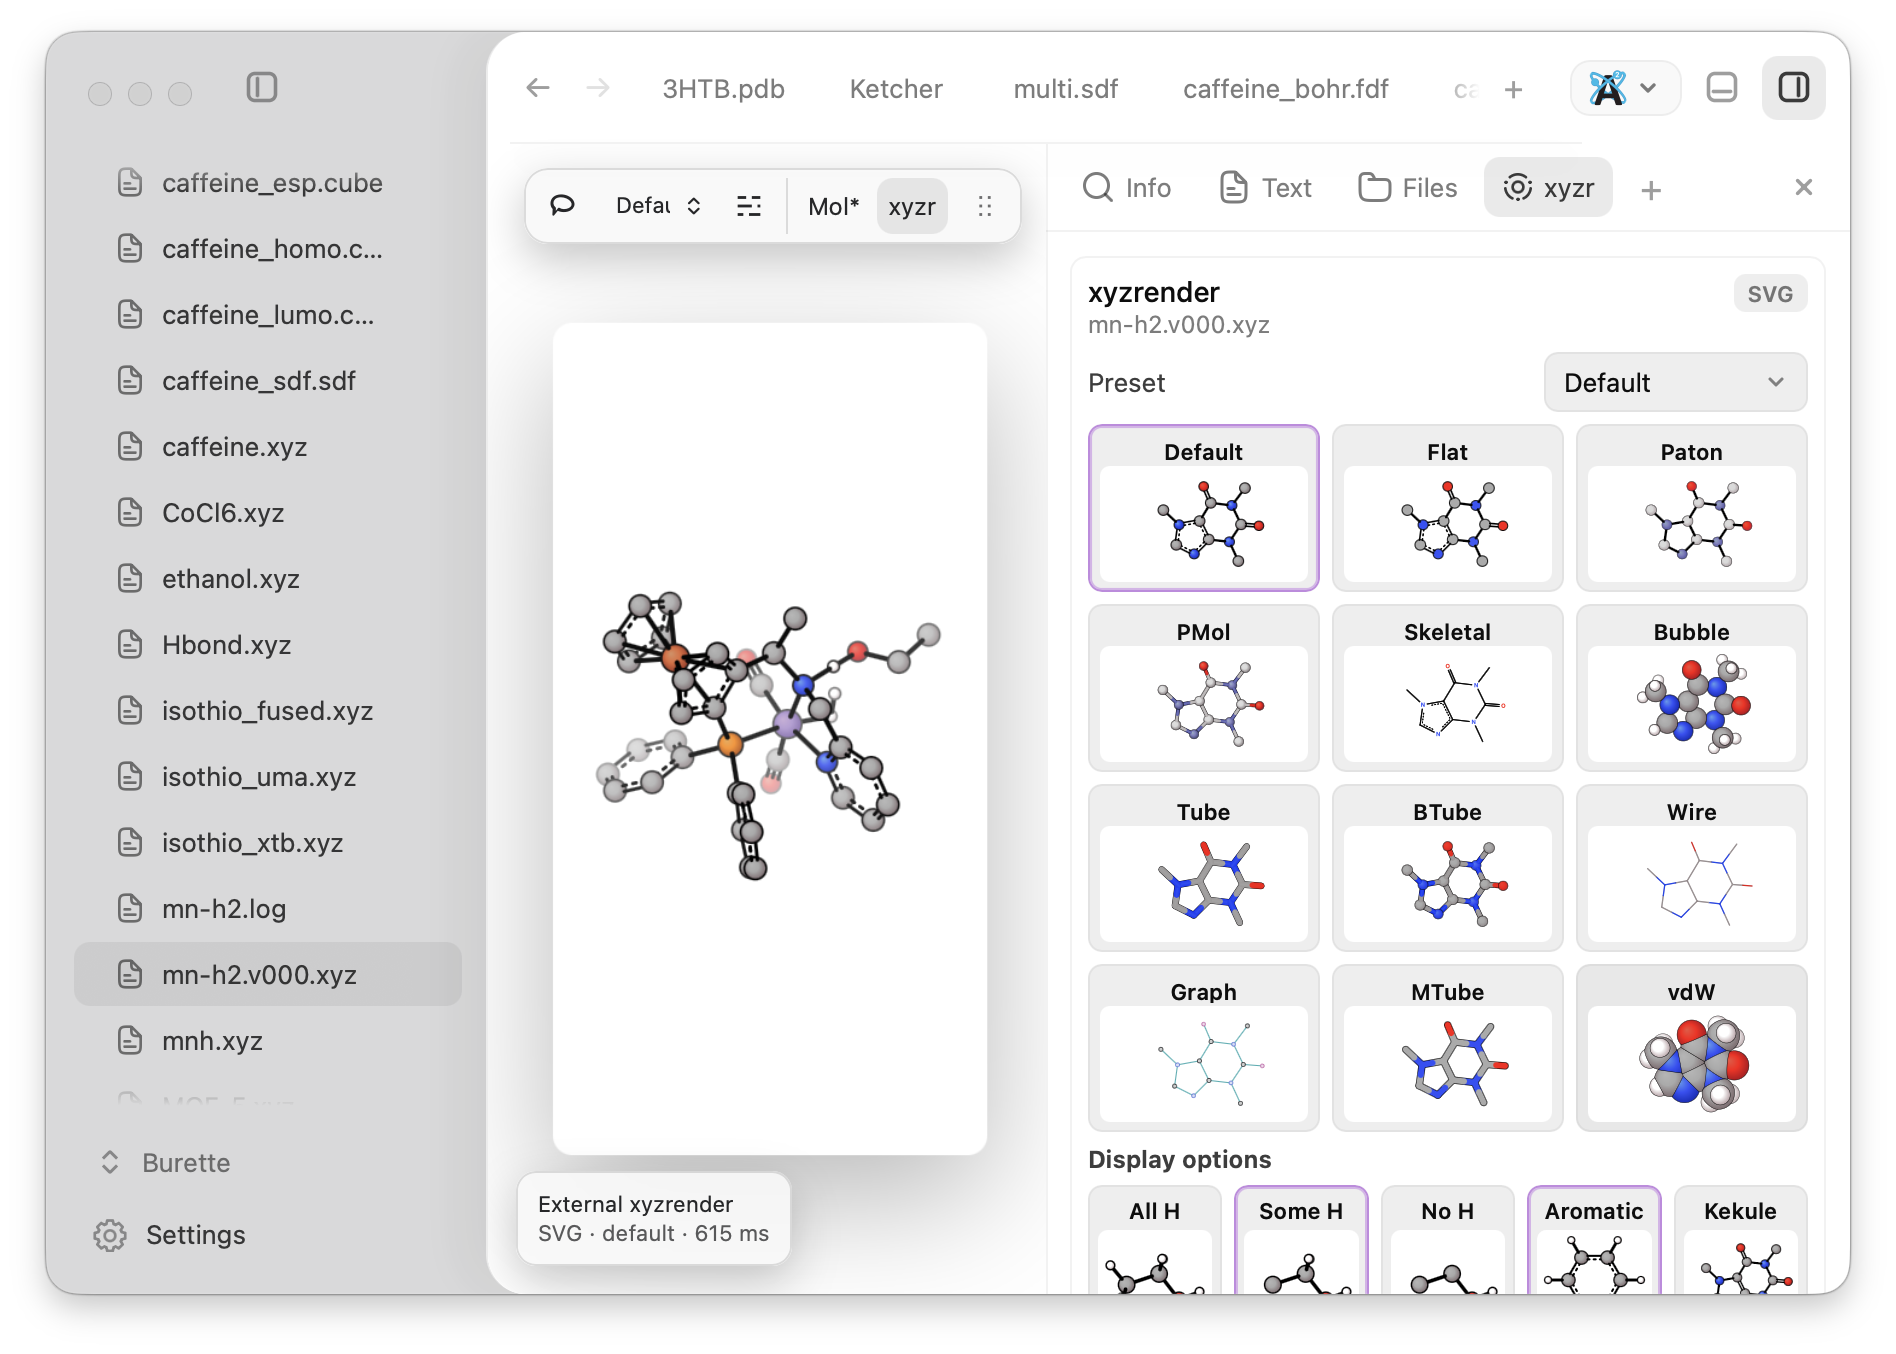
\includegraphics[width=0.92\linewidth]{Figure_4_xyzrender.png}
  \caption{Optional \texttt{xyzrender} adapter showing an SVG molecular preview
  and renderer presets alongside the local project file list.}
  \label{fig:xyzrender}
\end{figure}

Finally, an automated workflow can open one of these artifacts, inspect the
typed session state, request a defined viewer action, and place a bounded
markdown, table, or chart result in a docked panel. The machine-readable state
remains the primary verification channel; screenshots are reserved for visual
quality assurance.

\item \textbf{Impact}

Burrete's immediate impact is operational: it shortens the transition from a
generated file to an informed decision about the next tool. The same workspace
can expose a structure, a ligand table, a text log, and a specialized-renderer
handoff without implying that these artifacts share one scientific parser.
This is particularly useful in research pipelines that produce many
intermediate files and where provenance, renderer choice, and failed fallbacks
must remain visible.

The typed session boundary also creates a reproducible point of contact for
AI-assisted research software. An agent can query explicit document and viewer
state and invoke a limited action contract instead of inferring all state from
pixels. This enables research questions around auditable human--agent
inspection, cross-surface consistency, and bounded context for molecular
workflows without positioning the agent as an autonomous scientific
decision-maker.

The project is at an early adoption stage. On 10 July 2026, the public
repository reported 17 GitHub stars and 148 downloads of binary release assets
across releases; these are download events rather than unique-user counts
\cite{burrete}. The author is not aware of a peer-reviewed study that has yet
used Burrete as a research method, so no publication-impact claim is made.
Instead, the repository supplies source, published macOS release artifacts,
sample files, documentation, and contract tests so that prospective users and
reviewers can inspect the implementation and reproduce the illustrated
workflows.

\item \textbf{Conclusions}

Burrete combines Finder Quick Look, a persistent desktop workspace, a
source-built iPhone target, explicit molecular renderer adapters, and typed
agent sessions around local molecular files. Its contribution is the
integration boundary: the software makes established viewers and editors
available in a consistent inspection workflow while preserving which component
owns parsing, depiction, editing, or external visualization.

The current release is macOS-first; the iPhone target is experimental and
requires a source build. Optional external programs must be installed
separately, binary trajectories need appropriate paired context, and some
registered workflow artifacts deliberately fall back to text or metadata.
Future work will expand tested format coverage, collect public research-use
cases, and evaluate inspection workflows with independent users. These
limitations are preferable to overstating direct rendering or scientific
analysis that the software does not perform.

\end{enumerate}

\section*{Acknowledgements}

The author thanks the open-source communities behind Mol*, RDKit, Ketcher,
Tauri, \texttt{xyzrender}, and the other software cited in this article.

\section*{CRediT authorship contribution statement}

Sergei A. Nikolenko: Conceptualization, Methodology, Software, Validation,
Visualization, Project administration, Writing -- original draft, Writing --
review and editing.

\section*{Funding}

This work received no specific grant from funding agencies in the public,
commercial, or not-for-profit sectors.

\section*{Declaration of competing interest}

The author is the primary developer of Burrete and may benefit reputationally
from its adoption. The software is distributed under the MIT License. The
author declares no other competing interests.

\section*{Data availability}

No new research dataset was created for this article. Source code,
documentation, sample files, release artifacts, and the manuscript source are
available in the public GitHub repository \cite{burrete}.

\section*{Declaration of generative AI use}

Generative AI tools were used to assist with drafting and editing this
manuscript and with software-development workflows in the Burrete project. The
author checked claims against source-controlled code and documentation, revised
the generated material, and takes full responsibility for the final content.
No generative AI was used to create or alter the scientific screenshots or the
deterministic architecture diagram.

\bibliographystyle{elsarticle-num}
\bibliography{softwarex}

\section*{Current executable software version}

Version 1.0.22 is available from the GitHub release page:
\url{https://github.com/SergeiNikolenko/Burrete/releases/tag/v1.0.22}.
The release provides macOS DMG and ZIP artifacts; the iPhone target
is distributed as source code.

\end{document}
\endinput
